\documentclass[twoside,11pt,openright,a4paper]{report}

\usepackage{cstitle}
\usepackage[utf8]{inputenc}
\usepackage[american]{babel}
\usepackage{latexsym}
\usepackage{amssymb}
\usepackage{amsmath}
\usepackage{epsfig}
\usepackage[T1]{fontenc}
\usepackage{lmodern}
\usepackage{color}
\usepackage{datetime}
\usepackage{epstopdf}
\usepackage{hyperref}

\usepackage{csquotes}
\usepackage{listings}
\usepackage[backend=biber]{biblatex}

\usepackage{float}
\floatstyle{boxed}
\restylefloat{figure}

\addbibresource{refs.bib}

\hypersetup{
    pdfborder = {0 0 0}
}
\newcommand{\remark}[1]{{ \bf [ \footnotesize #1 ]}}
\newcommand{\Orangutan}{Orangutan}
\newcommand{\bibtex}{Bib{\TeX}}
\newcommand{\chapref}[1]{\textit{\nameref{#1}}}
\newcommand{\figref}[1]{Figure~\ref{#1}}

\graphicspath{ {graphics/} {./} }
% see http://imf.au.dk/system/latex/bog/

\begin{document}
\pagestyle{empty}
\pagenumbering{Alph}
\begin{titlepage}
\author{Rohde Fischer - 20052356}
\csAdvisor{Olivier Danvy}
\title{An automated approach\\to organizing {\bibtex}-files}
\maketitle

\end{titlepage}

%%%%%%%%%%%%%%%%%%%%%%%%%%%%%%%%%%%%%%%%%%%%%%%%%%%%%%%%%%%%%%%%%%%%%%%

\pagestyle{plain}
\setcounter{page}{1}

\chapter*{Abstract}
\addcontentsline{toc}{chapter}{Abstract}

%\chapter*{Acknowledgements}
%\addcontentsline{toc}{chapter}{Acknowledgments}
%
%\todo{\dots}
%
%\vspace{2ex}
%\begin{flushright}
%  \emph{Olivier Danvy,}\\
%  \emph{Aarhus, \today.}
%\end{flushright}
%
\tableofcontents

\pagenumbering{arabic}
\setcounter{secnumdepth}{2}

%%%%%%%%%%%%%%%%%%%%%%%%%%%%%%%%%%%%%%%%%%%%%%%%%%%%%%%%%%%%%%%%%%%%%%%

\chapter{{\bibtex}}
\label{ch:about}
\section{Introduction}
The goal of this chapter is to introduce {\bibtex}: the course of
events leading to {\bibtex} \chapref{sec:why_bibtex_came_to_be}, what
{\bibtex} is \chapref{sec:principles_of_bibtex}, how {\bibtex} is used
in principle \chapref{sec:practice_of_bibtex}, and how {\bibtex} is
used in practice \chapref{sec:how_bibtex_is_used_today}.


\section{Why {\bibtex} came to be}
\label{sec:why_bibtex_came_to_be}

The advent of {\TeX} has been a game changer for scientific writing,
witness the number of articles written in {\TeX} (or derivatives such
as {\LaTeX}).  For instance, on arXiv.org, nearly all articles are
formatted with \LaTeX.  Apart from being grateful to Donald Knuth for
providing such a robust system for scientific articles, writers can
also be thankful that {\TeX} has given the basis for Oren Patashnik
and Leslie Lamport to create {\bibtex} for managing scientific
bibliographies.

Before the wake of {\bibtex}, bibliographic references were managed
entirely by hand and required a lot of labor.  For instance, nearly
half of Mary-Claire van Leunen's book, \textit{A Handbook for
  Scholars}~\cite{leunen1992_handbook}, is dedicated to citing,
managing, and writing references, \ie, 150 pages out of 335 pages
(excluding the index).  Likewise, a significant fraction of Umberto
Eco's book, \textit{How to Write a Thesis}~\cite{eco1985_thesis}, is
also dedicated to managing and citing references and to ensuring a
proper bibliography.  All this manual labor has almost been made
obsolete by {\bibtex}.

Even more, {\bibtex} entries are now readily available online, and so
the practical problem of bibliographic references is now solved, in
principle.

\section{What is {\bibtex}}
\label{sec:principles_of_bibtex}

In the same spirit as {\LaTeX}, {\bibtex} is a simple software tool
for managing bibliographic references in scientific writing, using an
ASCII file to specify theses references.  Inside this ASCII file, the
components of each reference are specified, such as the author, title,
year and what kind of medium (\eg, a book or article) was used.  This
file will be referred to as \newdef{the {\bibtex} file} or
\newdef{\file{bib}}

Depending on the forum, there are differences in: how references
should be cited, be written, and the order in which they should be listed.
Each publisher has a mandatory setup.  The specific set of rules a
publisher has is referred to as a \newdef{bibliography style} or
\newdef{citing style}.

When processing a document, {\bibtex} cites according to the selected
bibliography style, ensures the formatting and the order in the
reference list, and ensures that only relevant entries are included.
The references are labeled consistently in the document according to
the citing style, the labels are used when a reference is cited and
these labels allows the reader to quickly find the reference in the
bibliography, as illustrated in \figref{fig:bibtex_example_alpha}.

Today, {\bibtex} has also enabled huge online resources with
references, automated extraction tools, sharing of references and easy
version control.  The {\bibtex} format is originally designed for use
with {\LaTeX}, but it has plugins for other formats as
well~\cite{bibtex_resource}.

\begin{figure}
  \centering
  
\includegraphics[width=0.8\textwidth]{bibtex-styles-ex-acm}
  \caption{{\bibtex} output using ACM citing style which uses numbers to
    index entries.  Source: ShareLaTeX~\cite{sharelatex2016_styles}}
\label{fig:bibtex_example_acm}
\end{figure}

\section{How {\bibtex} is used in principle}
\label{sec:practice_of_bibtex}

\subsection{Macro-use}

A {\bibtex} file consists of entries each corresponding to a
bibliographic reference, such as an article or a book.  Each entry in
turn contains meta information about the reference, through tags that
specify the kind of meta information such as the author or title.
Also, quite commonly, a file will contain a lot of shortenings for
text fragments that are reused.

To select the desired style the command
${\backslash}bibliographystyle$ is used, for example
${\backslash}bibliographystyle\{alpha\}$.  The style in turn controls
the formatting and how the references are labeled, as can be seen on
\figref{fig:bibtex_example_acm} and \figref{fig:bibtex_example_alpha}
where the labels are different, the abbreviation of author names are
different and some of the visual formatting is different.

To build a {\LaTeX}-document with {\bibtex} references in it, one
first runs the $latex$ command (or one of the derivatives) to produce
(among other things) an \file{aux}.  The \file{aux} contains auxiliary
information from the {\LaTeX}-compiler.  Then run the $bibtex$ command
which uses the \file{aux} to find the entries in use and to give them
labels according to the reference style.  The output from {\bibtex} is
a \file{bbl} with the formatted references, which is then used by
subsequent runs by {\LaTeX}, so the document will have labels at the
appropriate places and an bibliography in accordance with the labels.


\subsection{Micro-use}

Inside a {\bibtex} file, the format itself is fairly simple. At the
main level, we have $@STRING$, $@PREAMBLE$, $@COMMENT$ and $entries$.
$@STRING$ is for shortenings that can be used later in the {\bibtex}
file, $@PREAMBLE$ is for defining how to format the text and
$@COMMENT$ is for comments and $entries$.  The $entries$ correspond to
the different medium types, such as $@ARTICLE$, $@BOOK$ and
$@PROCEEDINGS$, which in turn contain the relevant tags for the given
entry.  Each entry consist of an identifying key and a set of tags.
The identifying key will be called \newdef{entry key} to avoid
ambiguity with the tag $key$.  For each entry type, there are a
specification of tags relevant to the given medium where some of them
are mandatory. For instance for an $@ARTICLE$ the tags $author$,
$title$, $year$ and $journal$ are mandatory and supplementary
information such as the $pages$ for the article and $volume$ of the
journal can be added.  For ease of use {\bibtex} provides predefined
strings for the months: $jan$, $feb$, $mar$ and so on.

Tags and entries are case insensitive. The literal content
(\newdef{text}) needs to be enclosed in either \{ and \} or quotes and
numbers can be written without.  $@STRING$ shortenings has to be
without quotes and curly brackets.  Concatenation of $@STRING$ and/or
text is done using \#~\cite{bibtex_resource}.  {\bibtex} is designed
to ignore unknown entries and tags, so it allows additional
information.  An example {\bibtex} file can be seen in
\figref{fig:bibtex_example}

\begin{figure}
  \centering
  \begin{small}
\begin{verbatim}
@String{JFP = "Journal of Functional Programming"}
@String{OUP = "Oxford University Press"}

@Article{abadi1991_substitutions
  author =      "Mart\'{\i}n Abadi and Luca Cardelli
                 and Pierre-Louis Curien
                 and Jean-Jacques L\'evy",
  title =       "Explicit substitutions",
  journal =     JFP,
  year =        1991,
  volume =      1,
  number =      4,
  pages =	"375--416",
  note =	"A preliminary version was presented at the Seventeenth
                 Annual {ACM} Symposium on Principles
                 of Programming Languages
                 (POPL 1990)"
}

@InBook{leunen1992_handbook,
  author =       "Mary-{C}laire van Leunen",
  title =        "A Handbook for Scholars",
  publisher =    OUP,
  year =         1992,
  pages =        "9--45,154--268"
}
\end{verbatim}
  \end{small}
  \caption{{\bibtex} example}
\label{fig:bibtex_example}
\end{figure}

When citing inside a {\LaTeX} file, the desired entry key from the
{\bibtex} is used inside the ${\backslash}cite$, for example if one
has a reference named $some\_article$ then the reference is used by
writing: ${\backslash}cite\{some\_article\}$.  To link the document
and the bibliography together the command ${\backslash}bibliography$
is used together with a parameter: the name the {\bibtex} file, for
example: ${\backslash}bibliography\{mybib\}$.

\begin{figure}
  \centering
  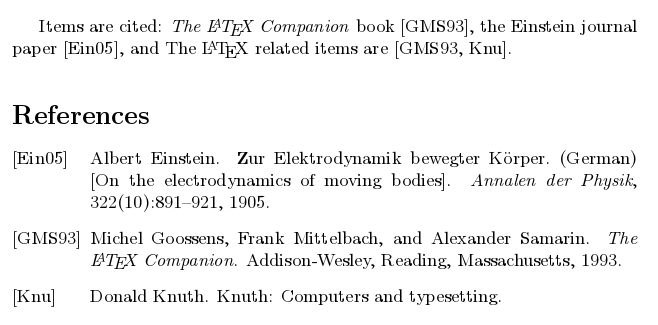
\includegraphics[width=0.8\textwidth]{bibtex-styles-ex-alpha}
  \caption{{\bibtex} output using alpha citation style which uses
    author names and year to index entries.  Source:
    ShareLaTeX~\cite{sharelatex2016_styles}}
\label{fig:bibtex_example_alpha}
\end{figure}


\section{How {\bibtex} is used in practice}
\label{sec:how_bibtex_is_used_today}

To this day, {\bibtex} is routinely used by researchers, witness that
almost all online resources for finding references provide {\bibtex}
output.  Many online databases are widely used to look up entries,
which has also given rise to a variety of ways to identify articles,
such as: arXiv numbers, DOI and ISSN.

Since {\bibtex} is capable of printing only the references used in a
{\LaTeX}-document, most people start using {\bibtex} as a database
having a complete file with the references they have used throughout
time.  A lot of people also find it practical to use their {\bibtex}
file as a way to keep track of what they read.

That {\bibtex} ignores unknown tags is used for de-facto standards, to
add additional information and to comment out tags by prefixing them
with $OPT$.  It is so widely used that is is common to see article
search engines make have tags that are not specified by {\bibtex} and
there is libraries that provide citing styles that make use of these
tags.


\section{Summary and conclusions}
\label{sec:about_conclusion}


{\bibtex} is a product of the advent of {\TeX} and the need for
managing bibliographic references.  The inside of a {\bibtex} file is
simple and intuitive, dividing the entries into types corresponding
to the medium it represents and having tags relevant to that medium.
{\bibtex} has become widely used and given rise to useful de-facto
standards and tools to assist with bibliographic references.

Like {\TeX}, {\bibtex} has been a game changer, and is something for
every scientific author to be happy about.  So has {\bibtex} solved the
problem of bibliographic references? It would seem so, had it not been
for Murphy's Law, as detailed in the next chapter.


%\remark{(Note to self:) should probably have half an eye on things
%  like: `G{\"o}del', when working with it}
%
%\remark{(Note to self:) people may use booktitle where title is
%  appropriate edition: The edition of a book---for example,
%  ``Second''. This should be an ordinal, and should have the first
%  letter capitalized, as shown here; the standard styles convert to
%  lower case when necessary~\cite{bibtex_description}.}
%
%\remark{http://tug2000.tug.org/TUGboat/Articles/tb24-1/patashnik.pdf}f

\chapter{The challenges in using {\bibtex}}
\label{ch:problem-description}
\rfquote{Anything that can go wrong, will go wrong.}{Murphy's Law}

\section{Introduction}
The goal of this chapter is to introduce the challenges of {\bibtex}
through concrete examples.  The terms of discourse, structural and
conjunctural, first defined
\chapref{sec:problems_structural_conjunctural}.  The rest of the
chapter is dedicated to problems with: duplicate entries
\chapref{sec:problems_duplicates}, spelling errors
\chapref{sec:problems_spelling}, covering the issues of initials
\chapref{sec:problems_initials}, online lookups
\chapref{sec:problems_look_ups}, name changes of forums
\chapref{sec:problems_name_changes}, de-facto standards and conformity
to the {\bibtex} specification \chapref{sec:problems_de_facto},
journal abbreviations \chapref{sec:problems_abbreviations}, {\bibtex}
strings that end up in the text
\chapref{sec:problems_strings_as_text}, inconsistent tags
\chapref{sec:problems_inconsistent_tags}, and inconsistent entry keys
\chapref{sec:problems_inconsistent_keys} .

\section{Structural vs. conjunctural issues}
\label{sec:problems_structural_conjunctural}

Unfortunately, even though {\bibtex} has made life a lot simpler for
scientific authors, it is far from perfect.  Inspired by economics,
the challenges in {\bibtex} can be divided into \emph{structural} and
\emph{conjunctural} issues.

\begin{itemize}
\item The \emph{structural} issues are the ones intrinsic to
  {\bibtex}: they are caused by its design, its standard tools, and
  missing information in {\bibtex} files.

\item The \emph{conjunctural} issues are the combination of
  circumstances, for instance if the source used does not contain
  complete information (\eg, extracting a reference from an article
  where the authors only have initials even though their full name is
  known) or the users having other practical priorities than assuring
  sound bibliographic references in their scientific writings.
\end{itemize}

Whether an issue is seen as conjunctural or structural is in part a
matter of opinion, as the definitions can be stretched in either
direction -- an issue also faced in economics.  Most of the issues are
arguably a combination of the two: as they could be fixed by careful
labor or by having the right tools available.  For example, most
bibliography managers have tools to switch between abbreviated and
full journal names.

Addressing the human factor, \ie, a conjunctural solution, is one
theoretically possible way for solving these issues.  One option would
be to ``simply'' motivate people to do things right.  Alas people are
not machines and thus this approach will be impossible in practice:
for most people, the interest is not the tools they use, but what they
use them for.  The interest in {\bibtex} is to ensure that their
documents contain appropriately many relevant references.

Since a conjunctural solution is not realistic, the goal is to provide
a structural solution to the issues.  In the perfect world, the
structural solution will be so complete that any issues left will be
entirely conjunctural, because one is either not using or misusing the
structural solution.


\section{Duplicate entries}
\label{sec:problems_duplicates}

When a group of authors is writing on the same document, work is often
divided and each author has their own \file{bib} that they use for
their references.  All might be fine until the group combines their
document and it turns out that multiple authors has used the same
reference, but with different keys, ending up having duplicate entries
in the bibliography.

Arguably it can be seen as a structural or a conjunctural problem.
The similarity of such entries will make them easier to spot with the
naked eye, arguably making a conjunctural solution relevant.  However
due to the similarity (at least if abbreviated the same way), a
structural solution is arguably also easy to make.  Making the problem
purely conjunctural would require a way to detect and merge these
entries.  Furthermore, if the entries use different key names, the
corresponding document should also be corrected. A challenge in this
case is when similar entries, that are still different entries, occur.

A similar issue happened in one of the drafts for this document: when
an author who wants to create a new entry copy and pastes an existing
entry, then giving the new entry an entry key, with intent to adjust
the contents.  This issue will also result in a duplicate entry, but
unlike the situation above, the duplicate should not be merged but
contain different content.

Having a tool that just merges duplicate entries may provide a
structural solution to the first case but will create a structural
issue in the second as it will automatically introduce new issues.
Thus the solution should not merge automatically.


\section{Spelling errors in general}
\label{sec:problems_spelling}

In almost, if not, all cases where people type text, spelling errors
will arise, sooner or later, \file{bib}s are no exception.  Extracting
meta-information automatically from documents may also run into a bad
extraction leading to spelling errors.  Furthermore, a spelling error
might not even be in the {\bibtex} document, as the misspelling can be
from the source, for instance if a title of a document is misspelled,
then the correct {\bibtex} will have to contain this error, as it is
the title of the source.

A user typing the entries manually is arguably the cause of spelling
errors.  Thus it can be argued that the issue is conjunctural, since
one could do a spell check.  However, one might also argue that
{\bibtex} should do a spell check.  In the case where automatic
extraction is the source of the spelling error the tool will give a
structural component to the issue.  Having a way of ensuring a spell
check and if such a way could ensure that the spelling error
corresponds to the source would make this issue conjunctural.


\section{Spelling errors in names}
\label{sec:problems_spelling_names}

Using a spell checker works for most entry tags, except names.  One
citing a name might get the name wrong and write ``Rene Rødhof
Hansen'' instead of ``René Rydhof Hansen''.  In this misspelling the
spell checker will be of no help.  The spell checker used in this
document suggests changing ``René'' to ``Rene'', which would introduce
a mistake.  Using a spell checker on names will be the cause of more
mistakes than corrections, and would thus cause a structural issue.
Providing a structural solution to misspelled names would require
either a spell checker that works for names or some database
containing valid names.


\section{Initials}
\label{sec:problems_initials}

Another issue in \figref{fig:conference_name} is the list of author
names that are so heavily abbreviated to initials that one cannot
realistically distinguish who the authors are.  This might originate
from the used citation style or from a resource where they are already
abbreviated.

If the initials come from the citation style, the issue is of a
structural nature.  However if it is copied from another source, or
just written like that, it is conjunctural, as the user did not ensure
full names.  A structural variant of the copying issue is if the
reference is copied by a tool, then it can be argued that such a tool
should try to detect initials.  Having a way to detect the initials
and the full names will provide a structural solution.  However, to
make an entirely structural solution a reliable way to know when the
initials are deliberate or not is needed.


\section{Online lookups}
\label{sec:problems_look_ups}

Many writers use online lookups for their bibliographic references.
In the Utopic case, all entries can be found online at all times.
Even though the databases out there are really good, erroneous results
can be found.  A lookup on Google Scholar in the beginning of February
2016 for: ``Results and Analysis of SyGuS-Comp’15'' can be seen in
\figref{fig:scholar_bad_result}, which contains an erroneous output.

\begin{figure}
  \centering
\begin{verbatim}
@article{alurresults,
  title={Results and Analysis of SyGuS-Comp’15},
  author={Alur, Rajeev and Fisman, Dana and Singh, Rishabh
          and Solar-Lezama, Armando}
}
\end{verbatim}
  \caption{Bad result from Google Scholar}
\label{fig:scholar_bad_result}
\end{figure}

Having found the article originally on arXiv.org the source of the
article is known to be EPTCS - Electronic Proceedings in Theoretical
Computer Science.  So not only does the Google Scholar result actually
not conform to the requirements of an article, the resource is in fact
not an article at all, but in the proceedings to a conference.
Finding the correct entry details at the EPTCS page reveals the entry
in \figref{fig:eptcs_lookup}.  Relying blindly on these being correct
causes a structural issue since the tools could automatically
introduce new errors.

The entries in those search engines cannot account for unpublished
work either, and expecting all published work to be represented in the
databases would be naive.  Having a reliable way to ensure that all
entries are present, however, is not a likely scenario.

Apart from the desire to detect erroneous entries from bad lookups,
using lookups for suggestions to most of the other issues can be a
useful part of a structural solution.  An optimal structural solution
to the bad lookups would be if it was possible to detect the users'
intended result.  As there is no way to know for certain what the user
intends, this is an Utopian idea.  A realistic idea would be to
provide a solution that limits the risk of bad lookups, which is only
a partial structural solution since the user would still have to
verify the result.

\begin{figure}
  \centering
\begin{small}
\begin{verbatim}
@Inproceedings{EPTCS202.3,
  author    = "Alur, Rajeev and Fisman, Dana  and Singh, Rishabh
               and Solar-Lezama, Armando",
  year      = "2016",
  title     = "Results and Analysis of SyGuS-Comp'15",
  editor    = "\v{C}ern\'y, Pavol and Kuncak, Viktor
               and Parthasarathy, Madhusudan"b,
  booktitle = "{\rm Proceedings Fourth Workshop on}
               Synthesis,
               {\rm San Francisco, CA, USA, 18th July 2015}",
  series    = "Electronic Proceedings in
               Theoretical Computer Science",
  volume    = "202",
  publisher = "Open Publishing Association",
  pages     = "3-26",
  doi       = "10.4204/EPTCS.202.3",
}
\end{verbatim}
\end{small}
  \caption{Correct lookup on EPTCS, after failed lookup on Google Scholar}
\label{fig:eptcs_lookup}
\end{figure}


% ref 3
\section{Name changes of forums}
\label{sec:problems_name_changes}

In \figref{fig:missing_org_scholar_lookup}, spotting the consistency
issues were relatively simple.  When looking at
\figref{fig:entry_journal_name_authors} it can be seen that the
conference name is slightly different in one of the entries, but so
close that they are probably the same conference.

\begin{figure}
  \centering
\begin{small}
\begin{verbatim}
\bibitem{stanifordchen96grids}
S.~S.-C. \emph{et al}.
\newblock {GrIDS} -- {A} graph-based intrusion detection system
          for large networks.
\newblock In {\em Proceedings of the 19th
          National Information Systems Security Conference},
          1996.

[...]

\bibitem{porras97emerald}
P.~A. Porras and P.~G. Neumann.
\newblock {EMERALD}: Event monitoring enabling responses
          to anomalous live disturbances.
\newblock In {\em Proc. 20th {NIST}-{NCSC}
          National Information Systems Security Conference},
          pages 353--365, 1997.

\end{verbatim}
\end{small}
  \caption{Inconsistent reference to the conference and heavily abbreviated author names}
\label{fig:entry_journal_name_authors}
\end{figure}

A visit to the homepage of the conference reveals that ``National
Information Systems Security Conference'' used to be named ``National
Computer Security Conference'', which is probably the reason for the
\texttt{\{NIST\}--\{NCSC\}} part of the first entry~\cite{nist2014_nissc}.  In
the same source it turns out that there are also references to the old
conference name, as seen in \figref{fig:conference_name}, so to
correctly identify potential inconsistencies, it should also recognize
name changes and variations.

\begin{figure}
  \centering
\begin{small}
\begin{verbatim}
\bibitem{snapp91dids}
S.~R.~S. \emph{et al}.
\newblock {DIDS} (distributed intrusion detection system) -
          motivation, architecture, and an early prototype.
\newblock In {\em Proceedings of the 14th
          National Computer Security Conference},
          pages 167--176, Washington, DC, 1991.
\end{verbatim}
\end{small}
  \caption{Name change of a conference}
\label{fig:conference_name}
\end{figure}

In {\bibtex}, there is no way of specifying that the same conference
has different names.  Therefore, there is a big structural part as
there is no support for identifying this issue.  Furthermore, the
owner of the {\bibtex} file might not even be aware of the issue,
which arguably could be conjunctural, since the user could do his
research, or structural, because the user should have a tool that can
assist him.  If a tool could reliably detect inconsistencies from the
same forum with different names, the name changes would become
conjunctural.


\section{De-facto standards and specification conformity}
\label{sec:problems_de_facto}

An interesting point is that not all the structural issues are bad.
There are practical ways to use the relaxed properties of {\bibtex}.
For instance {\bibtex} ignores unknown tags by design which is useful
in de-facto standards such as commenting entries out by prefixing with
$OPT$ or adding information that are not a part of the {\bibtex}
specification, such as ISSN and DOI.  The \texttt{crossref} tag is
technically not specified in {\bibtex}, but is still part of the tool.
In \figref{fig:mendeley_output}, an example is provided by a PhD
student from the Chemistry Department at Aarhus University.  This
example is created from Mendeley (see
Section~\ref{sec:related_mendeley}) and shows a lot of additional
information about the article.

\begin{figure}
  \centering
\begin{small}
\begin{verbatim}
@article{Acatrinei2003,
author = {Acatrinei, Alice I and Browne, D and Losovyj, Y B
          and Young, D P and Moldovan, M and Chan, Julia Y
          and Sprunger, P T and Kurtz, Richard L},
doi = {10.1088/0953-8984/15/33/101},
file = {:C$\backslash$:/Users/[...]pdf},
issn = {0953-8984},
journal = {Journal of Physics: Condensed Matter},
month = {aug},
number = {33},
pages = {L511--L517},
title = {{Angle-resolved photoemission study
          and first-principles calculation
          of the electronic structure of LaSb 2}},
url = {http://iopscience.iop.org/[...]},
volume = {15},
year = {2003}
}
\end{verbatim}
\end{small}
  \caption{Output from Mendeley containing additional information}
\label{fig:mendeley_output}
\end{figure}

This design choice is an issue, if strict conformity to the
specification is desired, as it is practical and widely in use, strict
validation would be counterproductive.  Some formatting styles make
use of unspecified tags, as can be seen in
\figref{fig:entry_with_issn}. It is interesting to find tags that are
not desired, \ie, tags that do not conform to the specification and
the de-facto standards.


%%
%% Internal ref 4
%%
\section{Journal abbreviations}
\label{sec:problems_abbreviations}

Most, if not all, journals require that journal names should be
abbreviated when publishing, especially those from competing
publishers.  However, internally in the {\bibtex} file the owner's
personal priorities are: consistent and correct naming.  As {\bibtex}
can be seen as a database of references, it makes sense to consider
full names as correct and the abbreviations to be a matter of
formatting.  Unfortunately, {\bibtex} does not handle abbreviations at
all, which for instance is apparent in articles from arXiv.org, as can
be seen in the bbl output in \figref{fig:inconsistent_naming}.

\begin{figure}
  \centering
\begin{small}
\begin{verbatim}
\bibitem[\protect\citename{Baroni \bgroup et al.\egroup }2014b]
          {baroni2014don}
          Marco Baroni, Georgiana Dinu, and Germ{\'a}n Kruszewski.
\newblock 2014b.
\newblock Don't count, predict!
          a systematic comparison of context-counting vs.
          context-predicting semantic vectors.
\newblock In {\em Proceedings of the 52nd Annual Meeting of
          the Association for Computational Linguistics},
          volume~1, pages 238--247.

\bibitem[\protect\citename{Bruni \bgroup et al.\egroup}2014]
          {bruni2014multimodal}
          Elia Bruni, Nam-Khanh Tran, and Marco Baroni.
\newblock 2014.
\newblock Multimodal distributional semantics.
\newblock {\em J. Artif. Intell. Res. (JAIR)}, 49:1--47.

[...]

\bibitem[\protect\citename{Collobert \bgroup et al.\egroup}2011]
          {collobert2011natural}
          Ronan Collobert, Jason Weston, L{\'e}on Bottou,
          Michael Karlen, Koray Kavukcuoglu, and Pavel Kuksa.
\newblock 2011.
\newblock Natural language processing (almost) from scratch.
\newblock {\em The Journal of Machine Learning Research},
          12:2493--2537.

[...]

\bibitem[\protect\citename{Kalchbrenner \bgroup et al.\egroup}2014]
          {kalchbrenner2014convolutional}
          Nal Kalchbrenner, Edward Grefenstette, and Phil Blunsom.
\newblock 2014.
\newblock A convolutional neural network for modelling sentences.
\newblock In {\em Proceedings of EMNLP}.
\end{verbatim}
\end{small}
  \caption{Inconsistent naming of journal and conference names}
\label{fig:inconsistent_naming}
\end{figure}

From the point of view that the style of {\bibtex} should format
abbreviations properly, the issue is structural.  In cases where the
abbreviation is wrong (\eg, due to a typo), the issue moves towards
being conjunctural, unless some kind of abbreviation specific spell
checker is being used.  Using full names and then formatting them
accordingly is the most sensible idea, since the style of abbreviation
could be interchanged, should the need arise: it is more readable and
it would create better conditions for output tools to provide
consistent formatting.

Currently there are multiple strategies for ensuring consistency in
abbreviations: some do a search and replace on the \file{bib}.  A bit
more structured one can use the strings in {\bibtex} to ensure a
consistent naming of a journal which can further be combined with the
usage of crossref.  Another approach is the use of Bib{\LaTeX} and
biber Section~\ref{sec:related_biblatex}, which provide the solution
in the formatting options~\cite{koppensteiner2011abbreviate}, provided
that the abbreviation handling of the style is correct.  This solution
causes the formatting issue to become conjunctural.  Bibliography
managers (see Section~\ref{sec:bibliography_managers}) tend to go with
the strategy of storing the references using full names.  When one
using a bibliography manager export to a {\bibtex} file (or another
format), the desired abbreviation style is applied to the export.
This strategy moves the issue towards being conjunctural, for the same
reasons as the Bib{\LaTeX} and biber solution.

As the purpose is to work on the {\bibtex} files, the formatting in
the end is technically not the primary concern.  Optimally the concern
is to ensure a consistent document.  Since {\bibtex} styles do not
take care of abbreviations, there is a need for considerations on how
to deal with consistency and to ensure the desired style of
abbreviations.  A partially structural solution ensures a consistent
structure, which can be modified according to the desired style of
abbreviations.  In a fully structural solution, the styles handle
abbreviations (such as the Bib{\LaTeX} and biber do).


\section{{\bibtex} strings ending up as text}
\label{sec:problems_strings_as_text}

When working with bibliographic references, {\bibtex} strings can
accidentally end up being textual content.  For instance if one, as
the PhD student earlier, exports from a program that does not make use
of the strings.  In the output from the aforementioned student seen in
\figref{fig:mendeley_output} the month is actually a text and not a
string as one would expect.  The use of text over strings prevents
re-use of fragments and localization.

When the usage as text over strings comes from a tool, such as in the
example above, the issue is of a structural nature.  When one types it
by accident then again it can arguably be both structural and
conjunctural.  Providing a structural solution to this would be by
being able to detect this and correct it.


%%
%% Internal ref 1
%% journal unknown oO
%%
\section{Inconsistent tags}
\label{sec:problems_inconsistent_tags}

Take the inconsistency in \figref{fig:entry_with_issn}, found in an
article on arXiv.org: two references from the same conference, but
with different years.  The inconsistency is easy to identify due to
the consistent content.  Correct and consistent content will help
tools in detecting inconsistencies.  This exposes a structural part of
the issue, as no such tools exist (to the authors' knowledge).

\begin{figure}
  \centering
  \begin{small}
\begin{verbatim}
\bibitem[Bernardy and Claessen(2015)]{bernardy_efficient_2015}
J.-P. Bernardy and K.~Claessen.
\newblock Efficient parallel and incremental parsing
          of practical context-free languages.
\newblock \emph{J. of Funct. Prog.}, 25, 2015.
\newblock ISSN 1469-7653.
\newblock \doi{10.1017/S0956796815000131}.

[...]

\bibitem[Mu et~al.(2009)Mu, Ko, and Jansson]{MuKoJansson2009AoPA}
S.-C. Mu, H.-S. Ko, and P.~Jansson.
\newblock Algebra of programming in {Agda}:
          dependent types for relational program derivation.
\newblock \emph{J. Funct. Program.}, 19:\penalty0 545--579, 2009.
\newblock \doi{10.1017/S0956796809007345}.
\end{verbatim}
  \end{small}
  \caption{Additional tag ISSN is provided in one of the entries}
\label{fig:entry_with_issn}
% consider the pages
\end{figure}

The ISSN might not exist for the \texttt{MuKoJansson2009AoPA}-entry.
In this case a structural detection system might be the cause of new
structural issue, either the removal of relevant data or forcing
entries when the data does not exist.  In this specific case, the
search result in \figref{fig:entry_issn_found} reveals that the
missing ISSN does exist and thus a tool pointing out the inconsistency
would in this case make the issue conjunctural.

% Source http://journals.cambridge.org/action/displayAbstract?fromPage=online&aid=6171388&fileId=S0956796809007345#
\begin{figure}
  \centering
\begin{verbatim}
@article{Mu:2009:APA:1630623.1630627,
 author = {Mu, Shin-cheng and Ko, Hsiang-shang
           and Jansson, Patrik},
 title = {Algebra of Programming in Agda:
          Dependent Types for Relational Program Derivation},
 journal = {J. Funct. Program.},
 issue_date = {September 2009},
 volume = {19},
 number = {5},
 month = sep,
 year = {2009},
 issn = {0956-7968},
 pages = {545--579},
 numpages = {35},
 url = {http://dx.doi.org/10.1017/S0956796809007345},
 doi = {10.1017/S0956796809007345},
 acmid = {1630627},
 publisher = {Cambridge University Press},
 address = {New York, NY, USA},
 }
\end{verbatim}
  \caption{Search revealing the ISSN}
\label{fig:entry_issn_found}
\end{figure}

%%
%% Internal ref 2
%% Source Electronic Proceedings in Theoretical Computer Science
%%

Provided a reliable way to lookup correct entries, a tool could move
the issues towards being conjunctural.  Take the inconsistency in
\figref{fig:inconsistent_proceedings} where two entries from the same
conference have different information.  One has an additional ``ICFP
'10'' and ``ACM'' in there, the other one does not.

\begin{figure}
  \centering
  \begin{small}
\begin{verbatim}
\bibitem[Bernardy and Claessen(2013)]{bernardy_efficient_2013}
J.-P. Bernardy and K.~Claessen.
\newblock Efficient divide-and-conquer parsing
          of practical context-free languages.
\newblock In \emph{Proc. of ICFP 2013}, pages 111--122, 2013.

[...]

\bibitem[Danielsson(2010)]{danielsson_total_2010}
N.~A. Danielsson.
\newblock Total parser combinators.
\newblock In \emph{Proc. of ICFP 2010}, ICFP '10,
          pages 285--296. ACM, 2010.
\end{verbatim}
  \end{small}
  \caption{Capt}
\label{fig:inconsistent_proceedings}
\end{figure}

An online search for {\bibtex} information gives the entries in
\figref{fig:missing_org_scholar_lookup} for the two articles, which
provides one possible option for a set of consistent entries.  As can
be seen, $ACM$ is the name of the organization and is probably missing
in the original {\bibtex} that produced the \file{bbl} inspected
above.  The Danielsson has additional information with the content
``ICFP '10'', which is not apparent in the search result.

\begin{figure}
  \centering
\begin{verbatim}
@inproceedings{bernardy2013efficient,
  title={Efficient divide-and-conquer parsing
         of practical context-free languages},
  author={Bernardy, Jean-Philippe and Claessen, Koen},
  booktitle={ACM SIGPLAN Notices},
  volume={48},
  number={9},
  pages={111--122},
  year={2013},
  organization={ACM}
}

@inproceedings{danielsson2010total,
  title={Total parser combinators},
  author={Danielsson, Nils Anders},
  booktitle={ACM Sigplan Notices},
  volume={45},
  number={9},
  pages={285--296},
  year={2010},
  organization={ACM}
}
\end{verbatim}
  \caption{Scholar lookup}
\label{fig:missing_org_scholar_lookup}
\end{figure}

\section{Inconsistent entry keys}
\label{sec:problems_inconsistent_keys}

The naming scheme for entry keys may vary throughout a \file{bib}.
For example, one of the users collaborating earlier might use entries
from various online databases getting keys corresponding to
\figref{fig:missing_org_scholar_lookup}, \figref{fig:eptcs_lookup} and
other structures in one big mess.  One of the users collaborating
might also be new to using {\bibtex} (could be a student learning) and
needs to find a nice an consistent way of writing the keys.

A challenge could be to avoid duplicate key names, which with a
consistent structure is more likely.  The duplicate entry keys can
have the advantage that it can be an indicator of a duplicate entry
Section~\ref{sec:problems_look_ups}.

Inconsistencies in keys might range from not a problem at all to fully
conjectural or structural, highly depending on the one's point of
view.  A user may simply not care and apart from the potential to
detect duplicate entries, may not feel a reason to.  In the
collaboration scenario, the additional way of detecting duplicates may
be valuable.  In this case, it arguably becomes conjunctural since the
authors should have agreed on a style - which might also have helped a
newcomer to have a good practice.  It can also be argued that it is
structural since {\bibtex} does not provide naming guidelines nor
tools for ensuring a guideline.

To make this issue structural, a naming convention would have to be
specified and some way of detecting deviations provided.  A blind
application of this method could result in two entries colliding with
the same key, requiring the attention of the user.


\section{Summary and conclusions}
\label{sec:problems_conclusion}

{\bibtex} has a lot of issues, for which a structural solution is
desired.  The problems covered are:

\begin{itemize}
\item Duplicate entries are not desired.  A structural solution will
  be to detect and merge duplicates, because a duplicate originating
  from missing or wrong data automatically merging may cause issues.

\item Spelling errors in general.  A structural solution will be able
  to find and correct the spelling errors, preferably by having the
  same spelling as published.  Alternatively, running a spell checker
  and having a way to account for deliberate misspellings, domain
  specific words and choice of language.

\item Spelling errors in names will challenge normal spell checkers.
  A structural solution is a spell checker that works for names or a
  database with names to verify names.

\item Use of initials can hide people's names to the level where
  finding a resource is hard.  A structural solution is to detect
  initials and the full names, accounting for when the initials are
  deliberate.

\item Online lookups can contain wrong data.  Optimally we can detect
  these wrong data reliably: the most realistic idea is to provide a
  way that limits the likelihood of erroneous results.

\item Name change of a forum which can affect detection of
  inconsistent tag use.  A structural solution will have some way of
  detecting when sources are from the same forum.

\item Conformity to de-facto standards and the {\bibtex} specification
  is desired, but should not prevent new de-facto standards.  A
  structural solution requires something that checks the conformity to
  a combination of specifications and de-facto standards accounting
  for changes in de-facto standards.

\item Journal abbreviations can be an issue for analyzing tools and
  having full names in {\bibtex} files.  A structural solution will be
  able to ensure that all entries are consistently abbreviated or
  de-abbreviated, preferably accounting for that people may want to
  switch between for formats.

\item {\bibtex} strings that end up as part of the text, can result in
  wrong data.  A structural solution will be able to detect and make
  text into strings when a string is desired.

\item Inconsistent tag usage in similar entries causes messy
  bibliographies. A structural solution will detect these
  inconsistencies and will be able to suggest a course of action.
  This solution may be challenged by deviations in information and
  forums that change name.

\item Inconsistent entry keys which can be an issue in collaboration
  and may make it harder to detect duplicates.  A structural solution
  could be to apply a naming scheme for the entry keys, accounting for
  similar entries that would result in identical entry keys.
\end{itemize}

With all these problems at hand, {\bibtex} may not seem like the
optimal tool after all.  What can be done with such a range of
issues?


\chapter{Our approach \remark{to {\bibtex}?}}
\label{ch:intro}
This dissertation documents a method for automated detection of
lexical and inconsistency concerns in {\bibtex} references.

\chapter{Related work}
\label{ch:related}
\section{Mendeley}

%%% Local Variables:
%%% mode: latex
%%% TeX-master: "thesis"
%%% End:


\chapter{Analyzing {\bibtex}}

\chapter{Organizing {\bibtex}-files}

\chapter{Conclusion and perspectives}
\label{ch:conclusion}

\todo{\dots}

%%%%%%%%%%%%%%%%%%%%%%%%%%%%%%%%%%%%%%%%%%%%%%%%%%%%%%%%%%%%%%%%%%%%%%%

\printbibliography{}
\end{document}
